\documentclass[informe.tex]{subfiles}
\begin{document}

Por la similitud que hay entre la función de transferencia realizable de un filtro digital y la función de transferencia realizable de un filtro analógico (funciones racionales, la primera en $z^{-1}$, y la segunda en s), los filtros IIR son versiones digitales de los diseños de filtros analógico.\newline

Aprovechando esta similitud, una técnica de diseño consiste en mapear la función racional en $s$ a otra función racional en  $z$.

\begin{figure}[h]
		\centering
		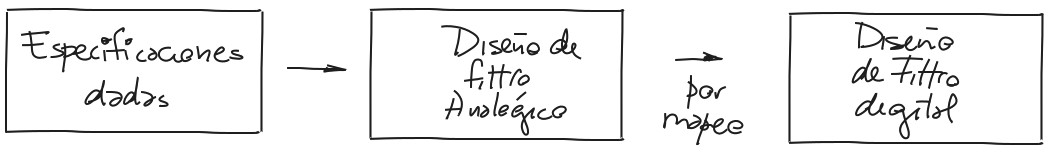
\includegraphics[scale=1.3]{filtro_digital_iir_1.jpg}
		\caption{Pasos para el diseño de filtros digitales}
		\label{fig:filtro_digital:iir:proceso}
		\end{figure}	

Por lo tanto el procedimiento, ilustrado en la Fig. \ref{fig:filtro_digital:iir:proceso}, se puede resumir en que las especificaciones del filtro se suelen dar en la frecuencia analógica para el tipo de filtro deseado, luego se sigue el procedimiento de diseño para un filtro analógico y por último, se mapea la función de transferencia desde el plano $s$ al plano $z$. Todo esto es siempre que se cumplan dos condiciones siguientes.\newline

1- Condición 1: \underline{Preservar las características en frecuencia de los filtros analógicos}. Significa que el eje $j\omega$ se mapea en el circulo unitario en el plano z, Fig. \ref{fig:filtro_digital:iir:cond1}.\newline
$$\begin{Bmatrix} s=j\omega | -\infty<\omega<\infty \end{Bmatrix} 
                   \mapsto 
  \begin{Bmatrix} z=e^{j\theta} |  -\pi < \theta  \leq \pi \end{Bmatrix}$$

\begin{figure}[h]
		\centering
		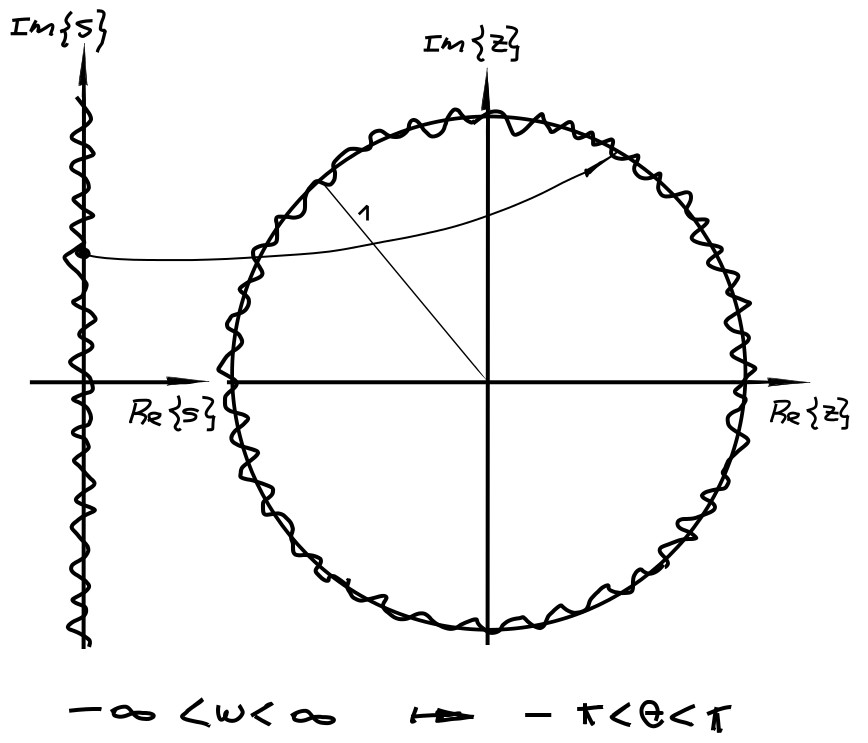
\includegraphics[scale=1]{filtro_digital_iir_2.jpg}
		\caption{Mapeo del eje  $j\omega$, en el plano s, en el circulo unitario, en el plano z}
		\label{fig:filtro_digital:iir:cond1}
		\end{figure}		
		
2- Condición 2: \underline{Preservar las propiedades de estabilidad}. Para un sistema estable en s, no debería haber polos en el semiplano derecho, de forma equivalente para un sistema digital, los polos no deberían estar fuera del circulo unitario, Fig. \ref{fig:filtro_digital:iir:cond2}
    $$\begin{Bmatrix} s / Re[s]<0 x \end{Bmatrix} 
              \mapsto 
      \begin{Bmatrix} z /  |z|<1 \end{Bmatrix}
    $$

\begin{figure}[h]
		\centering
		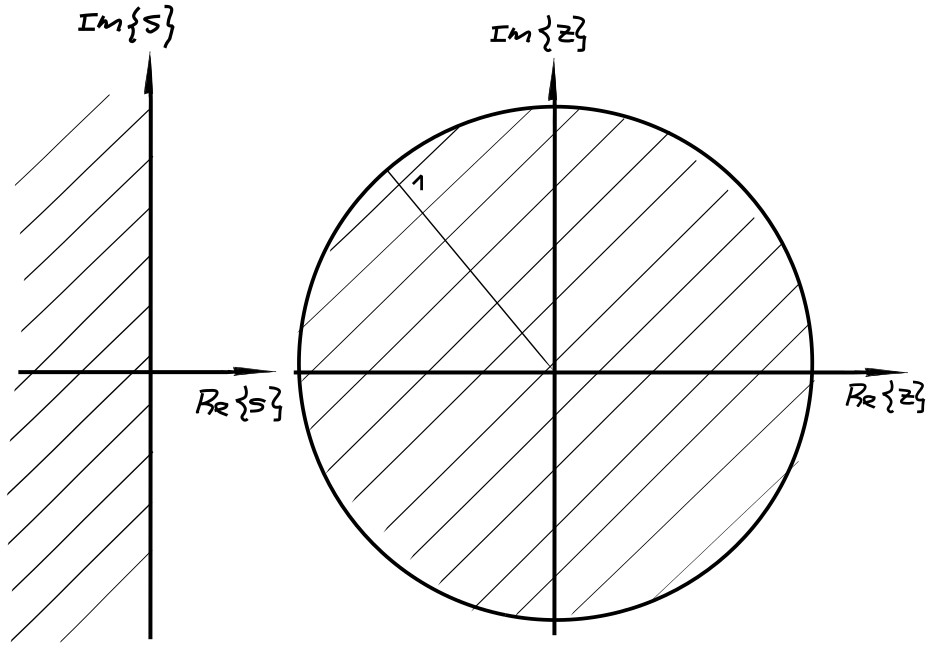
\includegraphics[scale=1]{filtro_digital_iir_3.jpg}
		\caption{Mapeo del semiplano izquierdo del plano s dentro del circulo unitario en el plano z}
		\label{fig:filtro_digital:iir:cond2}
		\end{figure}	
		

\newpage\subsection{Transformación por Método de Euler}
{
Este método de mapeo es uno de los métodos por integración numérica, surge de aproximar la derivada en tiempo continuo mediante algunas diferencias diferencias finitas. El efecto resultante es reemplazar una ecuación diferencial (caracterización de un filtro analógico) con una ecuación de diferencias (caracterización de un filtro digital).\newline

\textbf{Función de mapeo}\newline

	El método de aproximación de Euler consiste en aproximar la derivada en tiempo continuo con un diferencia de primer orden 

		$$
			\left. \frac{d y(t)}{dt} \right|_{t=nT} = \frac{y(n)-y(n-1)}{T}
		$$

quedando como resultado la función de mapeo, $s=f(z)$, desde el plano s al plano z como:
		$$
			s = \frac{1-z^-{1}}{T} \triangleq f(z)			
		$$
donde $T$ es el periodo de muestreo, y para el caso de expresar la relación inversa sería
		$$
			z = \frac{1}{1-sT}
		$$

\underline{Desarrollo:}
		$$
			\left. \frac{ d \hat{ y(t) } }{dt} \right|_{t=nT} 
			=
			\frac{y(n)-y(n-1)}{T}
				\xleftrightarrow[]{\mathscr{L}}						
			sY(s)= \frac{ Y\left(z^{-1}\right) - z^{-1} Y(z^{-1})}{ T }
		$$
		$$
			y(k)= \left. \hat{t} \right|_{t=nT} 
				\xleftrightarrow[]{\mathscr{L}}
				sY(s) = \frac{1-z^{-1}}{T}Y(z)
		$$\newline

\textbf{Verificación de las condiciones de mapeo:}\newline

1- Condición 1: conservación de las características de frecuencia. Mapear el eje $j\omega$ en el plano z resulta en la siguiente expresión 

		$$(z-1/2)=1/2 \cdot e^{j2\cdot atan(\omega T) }$$
		
		\begin{figure}[h!]
		\centering
		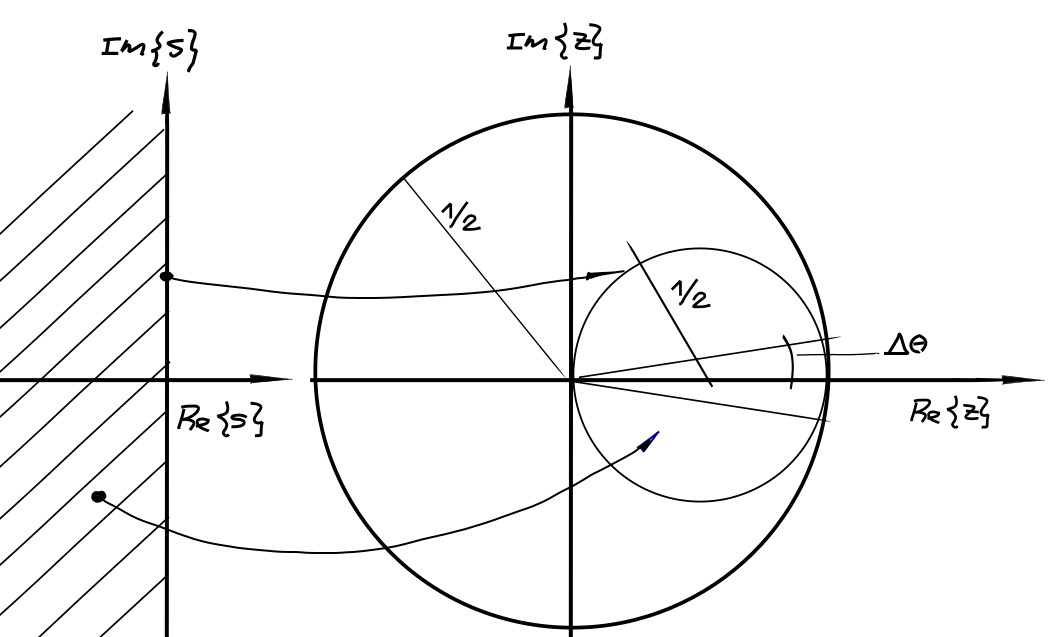
\includegraphics[scale=1]{iir_metodo_euler_1.jpg}
		\caption{Transformación por método de Euler. Mapeo del eje $j\omega$ en el plano z}
		\label{fig:filtro_digital:iir:invariante_1}
		\end{figure}	
				
Como se ve en la Fig. \ref{fig:filtro_digital:iir:invariante_1} no se cumple la condición, porque no queda circunscrito en el circulo unitario. Pero también se observa que para \underline{un $\Delta \theta=\omega T$ pequeño el mapeo resulta en una buena aproximación de la condición 1}.\newline

2- La condición 2: para preservar la características de estabilidad implica que el semiplano izquierdo $Real[s] \leq 0$ quede mapeado dentro del circulo unitario, $|z|<1$. Se verifica ésta condición mediante la siguiente expresión:
		$$
			\left| z \right| 
			= 
			\left. \left| \frac{1}{1-sT} \right| \right|_{s=\sigma + j \omega}
			=
			\frac{
					1
			   }{
			   		\sqrt{ \left(1+T\sigma \right)^2 + \left(T\omega \right)^2}
			   }
			   <1
		$$		
		
}

%%
\newpage
\subsection{Transformación invariante al impulso }
{
Este procedimiento asegura que la respuesta al impulso del filtro digital $h(n)$ resultante sea la versión muestreada de la respuesta al impulso correspondiente filtro analógico $\hat{h}(t)$ 
		$$h(n) \triangleq \left. \hat{h}(t) \right|_{t=nT} $$ 

donde $T$ es el periodo de muestreo.\newline


\textbf{Función de mapeo}\newline

La función de mapeo queda establecida como
$$ 
			z = e^{sT} \rightarrow \theta = \omega T
		$$ 
donde $\theta$ es la frecuencia digital, y esta comprendida entre $|\theta| \leq \pi$.\\

La función de mapeo surge de comparar ambas respuestas en frecuencia
	$$
		\begin{matrix}
			\sum_{i=0}^{\infty} \frac{\hat{ \xi }_i  }
			                      { s + \hat{p}_i } 
			 &  
			 \longrightarrow 
			 &
			\underbrace{
					\sum_{i=0}^{\infty} \frac{ \hat{ \xi }_i }{ 1 - e^{ \hat{p}_i T} z^{-1} }
					=
					\sum_{i=0}^{\infty} \frac{ \hat{ \xi }_i }{ 1 - p_i z^{-1} }
				}
			\\
			& &
	        p_i=e^{\hat{p}_i T}	
		\end{matrix} 
	$$

resultando que el polo en el plano s, $\hat{p}_i$, queda mapeado en el plano z como $p_i=e^{\hat{p}_i T}$.\\
		
		
\underline{Desarrollo:}\\

Para un par transformado de la respuesta al impulso $\hat{h}(t)$

	\begin{equation}
		\label{eqn:iir:invariante:func_1}	
		\hat{h}(t) = \sum_{i=1}^{N} \hat{ \xi }_i e^{ \hat{p}_i t} \hat{u}(t)
		\xleftrightarrow[]{\mathscr{L}}
		\hat{H}(s)=\sum_{i=1}^{N}{ \frac{ \hat{\xi}_i}
									{ s + \hat{p}_i }}
	\end{equation}
	
muestreando la $\hat{h}(t)$ a intervalos regulares $T$ se tiene que

	\begin{equation}
		\label{eqn:iir:invariante:func_2}	
		h(n) =  \left. \hat{h}(t) \right|_{t=nT} 
		           = \sum_{i=1}^{N} \hat{ \xi }_i e^{ \hat{p}_i n T} u(n)
		\xleftrightarrow[]{\mathscr{Z}}
		H(z) = \sum_{i=1}^{N}
		               { \frac{\hat{\xi}_i}
		                      { 1 - p_i z^{-1}}}		           	
	\end{equation}

Comparando ambos resultados de \ref{eqn:iir:invariante:func_1} y de \ref{eqn:iir:invariante:func_2} se llega a
	$$
		p_i=e^{\hat{p}_i T}
	$$
donde $p_i$	 es el polo $i$ en el plano z correspondiente al polo equivalente $\hat{p}_i$ en el plano s.\newline 


\textbf{Verificación de las condiciones de mapeo:}\\
 	
La característica de frecuencia de la secuencia muestreada, $x(n)$, es una suma escalada de un número infinito de copias desplazadas en frecuencia de la característica de frecuencia de la correspondiente señal de tiempo continuo $x(t)$

	$$
		X(e^{j\theta})
		=
		\left.		            
		\frac{1}{T} \sum_{k=-\infty}^{\infty}
		          { \hat{X} \left(
		                 j \left( 
		                       \frac{\theta}
		                             {T}
								+
								\frac{2 \pi k}
		                             {T}		                             
		                  \right)
		           \right)}
		\right |_{\omega T = \theta}
      =
		\frac{1}{T} \sum_{k=-\infty}^{\infty}
		          { \hat{X} \left(
		                 j \left( 
		                       \omega
								+
								\frac{2 \pi k}
		                             {T}		                             
		                  \right)
		           \right)}      
	$$
			
Gráficamente se puede ver en la Fig. \ref{fig:iir:invariante_1_2} que el mapeo del plano s al plano z resulta en tiras del plano s dentro del circulo unitario, quedando estas en una misma región en z. Por lo tanto, el mapeo no es lineal, es decir que hay más de un punto del plano s que se mapea en un mismo punto en el plano z.\newline

	\begin{figure}[h!]
	\centering
	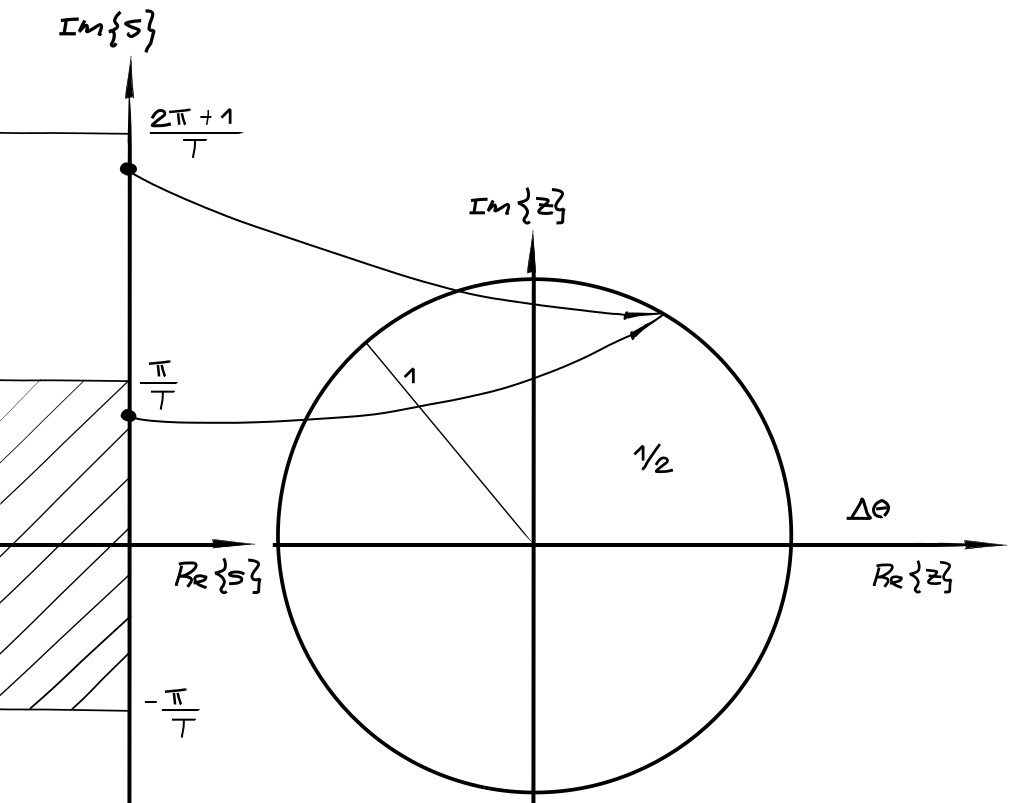
\includegraphics[scale=1]{iir_invariante_cond_5.jpg}	
	\caption{Transformación invariante al impulso. Mapeo resultante en el plano z}
	\label{fig:iir:invariante_1_2}
	\end{figure}	

Por lo tanto solo es aplicable a señales de banda limitada que cumplen la condición		
	$ | \hat{H}(j\omega) | \simeq 0  $ para $|\omega|>\omega_B$.
Si no se cumple esa condición ocurre un solapamiento (o aliasing) de las regiones.\\

\underline{Desarrollo:}\\	 

Primeramente, para ver la relación entre la respuesta en la frecuencia digital, $X\left( e^{j\theta} \right)$	y la respuesta en frecuencia analógica, $\hat{X}\left( j\omega \right)$ se plantea la transformada de Fourier de la señal muestreada $\hat{x} (nT)$. Así que primero se presenta la señal muestreada como un tren de impulsos equis espaciados y escalado de $x(nT)$ y luego a ésta se le aplica la transformada de Fourier.
	
	\begin{center}
	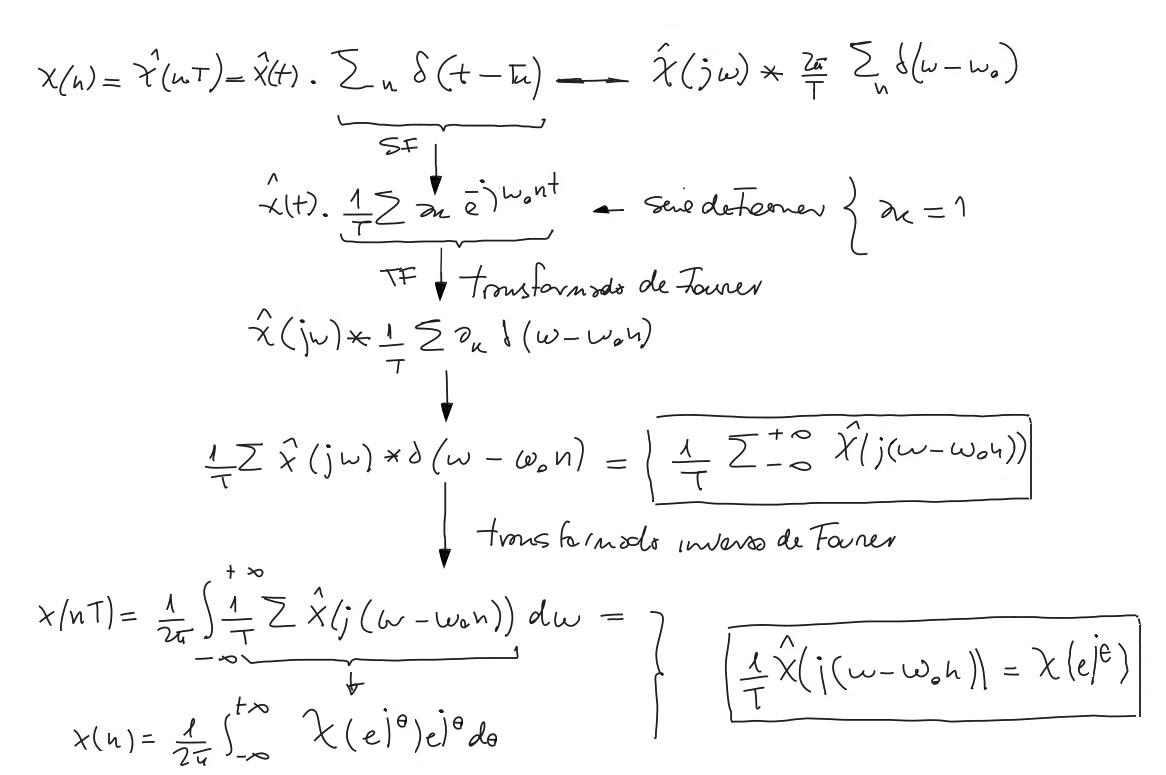
\includegraphics[scale=1.1]{iir_invariante_cond_1.jpg}	
	\end{center}

así se llega a que la respuesta en frecuencia digital, que es la sumatoria de las respuestas analógicas escaladas en $1/T$ y desplazada en múltiplos enteros de $\omega_0=\frac{2\pi}{T}$ 

	\begin{center}
	$ 
	   \frac{1}{T} \hat{X}\left( j(\omega - \omega_0 n) \right)
	   = 
	   X\left( e^{j \theta } \right)
	$
	para 
	$ |\theta | \leq \pi $
	\end{center}
	
Segundo, si se parte de la respuesta al impulso analógica $\hat{h}(t)$ se debería llegar a la misma relación. Esto es,
	$$
		x(t)|_{t=nT} = \frac{1}{2\pi}
		               \left.
		               \int^{-\infty}_{\infty}
		                    { \hat{X} \left( j\omega \right) e^{j \omega t} d \omega }
		               \right|_{t=nT}
	$$

y luego desarrollando esta expresión tal como 

	\begin{center}
	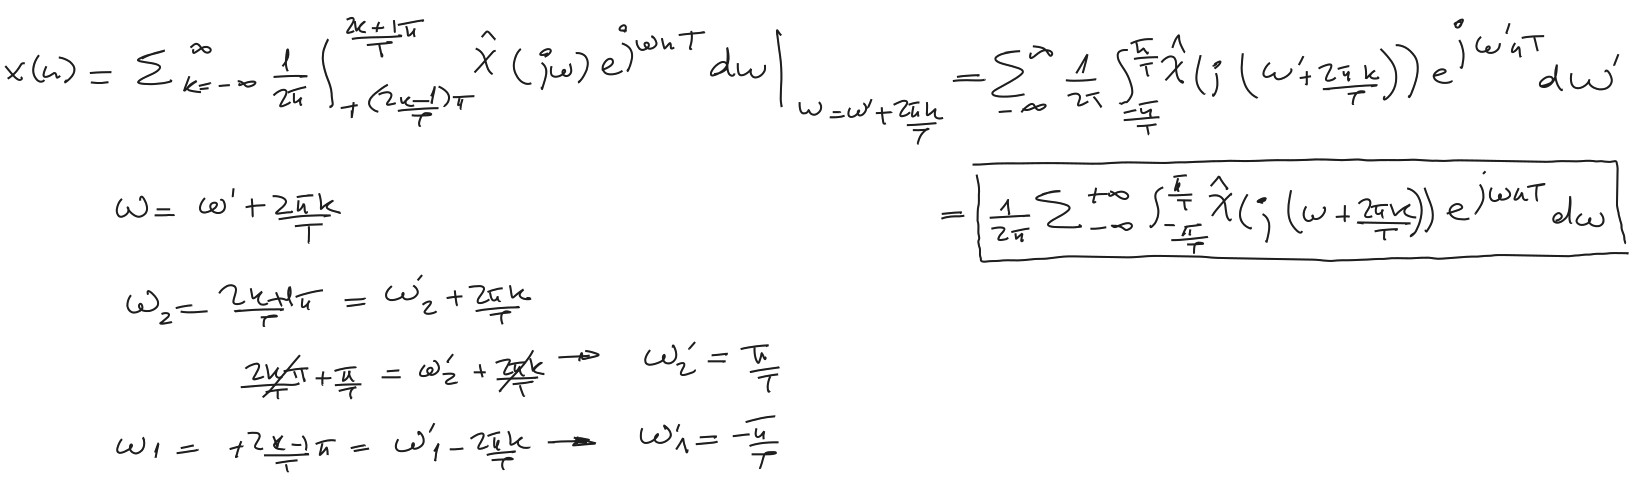
\includegraphics[scale=1.1]{iir_invariante_cond_2.jpg}
	\end{center}
	
mediante un cambio de variable queda que

	$$\begin{matrix}
	

		x(n) & = \left.
		        \frac{1}{2\pi}
			    \sum_{k=-\infty}^{\infty}
			    \int_{k=\frac{2k-1}{T}\pi}^{\frac{2k+1}{T}\pi}
			       {\hat{X}\left( j\left(\omega + \frac{2\pi k}{T} \right) \right)}
			  \right|_
			          {
			           \begin{matrix}
			           		\omega T = \theta \\
			           		\omega_1 T = \theta_2 \\			           		 
			           		-\omega_1 T = \theta_1	\\		           		
					   \end{matrix}
			          } 
  		 \\
            & =  \frac{1}{2\pi}
                 \sum_{k=-\infty}^{\infty}
                 \int_{-\pi}^{\pi}
                   { 
                     \hat{X} \left( j \left( \frac{\theta}{T} + \frac{2\pi k}{T} 
		                      \right) \right)
		             e^{j n \theta }
		             \frac{ d \theta }{T}
                   }
		\end{matrix}         
	$$
		
y finalmente se pueden relacionar ambas características en frecuencia como:
	
	\begin{center}
	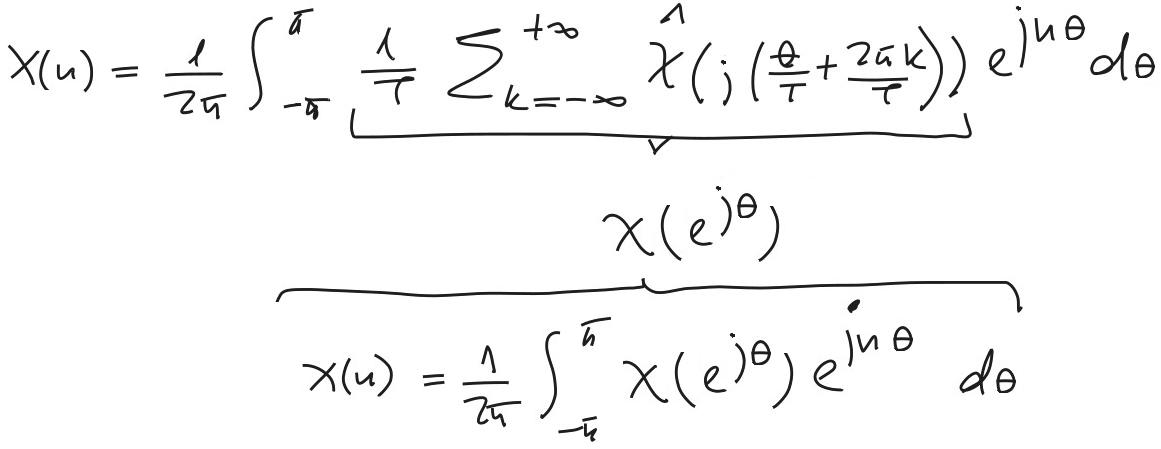
\includegraphics[scale=0.8]{iir_invariante_cond_3.jpg}		
	\end{center}
}			
		
\newpage
\subsection{Transformación por mapeo bilineal}
{
\textbf{Función de mapeo:}\newline
Se define a partir de la siguiente función de mapeo
	$$
	s=f(z)= \frac{2}{T}
	        \frac{1-z^{-1}}{1+z^{-1}}
	$$
y la relación inversa
	\begin{center}
	$
		z=\frac{2+sT}{2-sT}
	$
	o de forma equivalente
	$
		z^{-1}=\frac{2-sT}{2+sT}
	$		
	\end{center}	
 y la relación entre la frecuencia digital y analógica
	$$
		\theta(\omega) = atan \left( 
								\frac{4\omega T}
									 {4-(\omega T)^2}
							 \right)
	$$

\textbf{Verificación de las condiciones de mapeo:}\\

De la condición 1, el eje $j\omega$ queda mapeado en el circulo unitario, así que cumple dicha condición de conservar las características en frecuencia. Y de la condición 2, la región del semiplano izquierdo del plano s queda dentro del circulo unitario en el plano z, Fig. \ref{fig:iir:bilineal_1_2}

	\begin{figure}[h!]
	\centering
	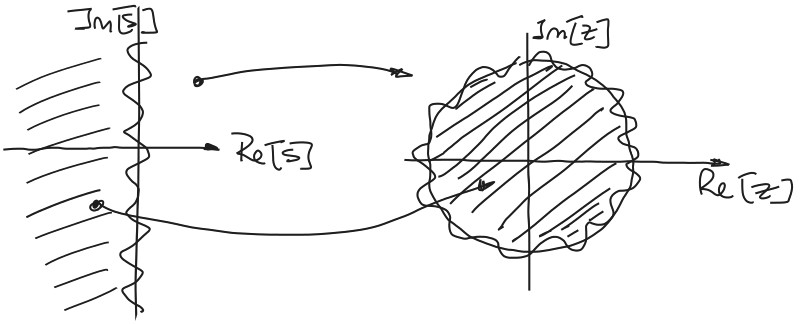
\includegraphics[scale=1]{iir_bilineal_mapeo.jpg}	
	\caption{Transformación bilineal. Mapeo resultante en el plano z}
	\label{fig:iir:bilineal_1_2}
	\end{figure}	

\underline{Desarrollo:} \newline 	 
1- La condición de que se conservan las características de frecuencia sale de reemplazar  $s=j\omega$ en
	$$
		z = \frac{ 2 + j\omega T}
		         { 2 - j\omega T}
		  = 
		  e^{ 
		     atan \left( \frac{ 4 \omega T}
		               { 4 - (\omega T)^2}
		          \right)
		   }
		 = 
		 e^{j \theta(\omega)}
	$$
quedando finalmente 
	$$
		\theta(\omega) = atan \left( 
								\frac{4\omega T}
									 {4-(\omega T)^2}
							 \right)	
	$$
2- De igual manera, pero ahora con $\sigma \neq 0$ se tiene que $s=\sigma + j\omega$	y por lo tanto
	$$
		z = \left. \frac{ 2 + j\omega T}
		         { 2 - j\omega T} \right|_{s=\sigma + j\omega}
		  = 
		  \frac{ 2 + \sigma T + j \omega T }{ 2 - \sigma T - j \omega T }		  		
    $$		 
si $Real(s)=\sigma <0$ entonces $|z|<1$, de esta manera se concluye que también cumple la condición 2. Quedando representado el mapeo en z como se muestra en la Fig. \ref{fig:iir:bilineal_1_2}.\newline


\textbf{Función de transferencia y respuesta en frecuencia} \newline 	

Como se vio en el desarrollo de las condiciones de mapeo, para preservar las características de frecuencia y estabilidad éste mapeo bilineal cumple con ambas propiedades, quedando relacionadas de la siguiente mantera ambas respuestas en frecuencia.
	$$
		H(z) = \left. \hat{H}(s) \right|_{
											s=(2/T)(1-z^{-1})/(1+z^{-1})
										}
	$$
donde $T$ es el período de muestreo.

Pero la relación entre las frecuencia digital $\theta$ y la frecuencia analógica $\omega$ no es uniforme, Fig. \ref{fig:iir:bilineal:relacion_w_theta_1}, esto es
	$$
		s=\sigma + j \omega
		 = \frac{2}{T} \frac{1-e^{-j \theta}}{1+e^{-j\theta}}
		 = j \frac{2}{T} tan \frac{\theta}{2}
		 \begin{cases} 
		 	\omega = \frac{2}{T} tan \frac{\theta}{2}
		 	\\
		 	\sigma=0		 	
		 \end{cases}
	$$

	\begin{figure}[h!]
	\centering
	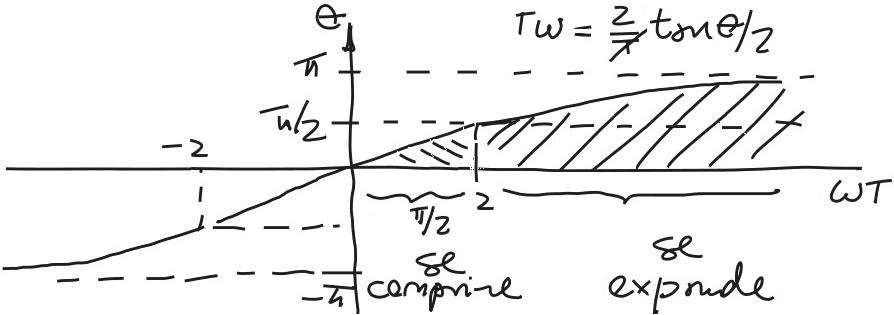
\includegraphics[scale=1]{iir_bilineal_w_theta.jpg}	
	\caption{Transformación bilineal. Relación entre la frecuencia analógica  $\omega$ y la frecuencia digital $\theta$}
	\label{fig:iir:bilineal:relacion_w_theta_1}
	\end{figure}	

\textbf{Predistorsión – prewarping}\\

La predistorsión es un procedimiento que consiste en encontrar una constante o una frecuencia de muestreo $\omega_s = \frac{2\pi}{T}$ equivalente, tal que dada una frecuencia analógica, $\omega_x$, coincida con el mapeo inverso de una frecuencia digital relacionada linealmente con esta frecuencia analógica dada.\newline
	$$
	     \omega_x T'/2 = \left.  tan \left( \frac{\theta}
	                                      {2} 
	                     \right) \right|_{\theta = \omega_x T/2}
	$$

Ya que para la frecuencia de muestreo utilizada, $\omega T<\pi/2$, las frecuencias analógica se comprimen, y $\omega T>\pi/2$ las frecuencias expanden respecto a la frecuencia analógica, Fig. \ref{fig:iir:bilineal:relacion_w_theta_1}.\newline

	\begin{figure}[h]
		\centering
		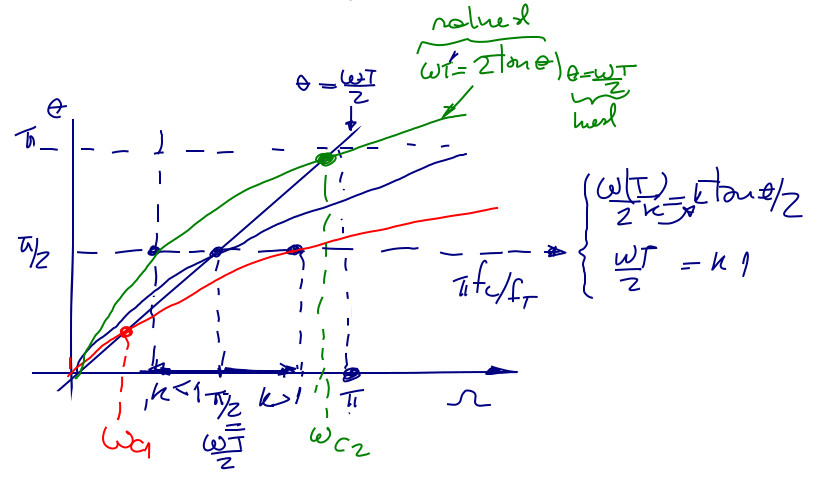
\includegraphics[scale=1.3]{iir_bilineal_warping.jpg}	
		\caption{Transformación bilineal. Relación entre la frecuencia analógica  $\omega$ y la frecuencia digital $\theta$}
		\label{fig:iir:bilineal:relacion_w_theta_2}
	\end{figure}	
	
Entonces, se busca un punto donde coincida la relación lineal con la relación binomial, Fig. \ref{fig:iir:bilineal:relacion_w_theta_2}.\newline
 
A continuación se busca una frecuencia equivalente de muestreo tal que se relacionen esta dos relaciones lineal y no lineal (intersección de los dos puntos.)\newline

\begin{center}
	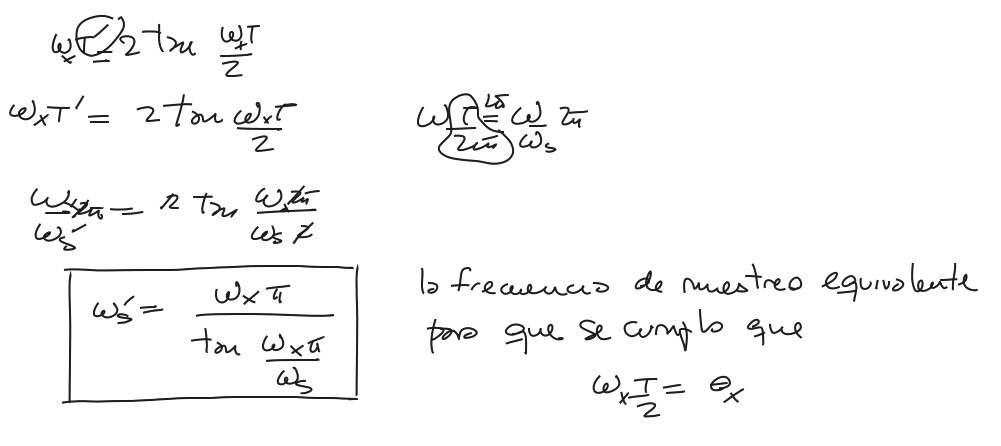
\includegraphics[scale=1.2]{iir_bilineal_warping2.jpg}	
\end{center}

}
\end{document}	
